\begin{appendices}
    \section{Benchmarking Code}\label{code}
    \subsection{Performance Benchmark}
    \subsubsection{Python vs. Cython Benchmark}
    \begin{minted}[mathescape,linenos,frame=lines]{python}
    # Importing Dependencies
    import amsimp
    import time
    import csv
    import os
    import random
    
    # ---------------------------------------------------#
    
    # Output filename.
    filename = input("The name of the CSV file: ")
    filename = filename + ".csv"
    
    # Creates a CSV file.
    def csv_file():
        file = os.path.isfile(filename)
        csvfile = open(filename, "a")
    
        fieldnames = ["detail_level", "time"]
        writer = csv.DictWriter(
            csvfile, delimiter=",", lineterminator="\n", fieldnames=fieldnames
        )
    
        if not file:
            writer.writeheader()
    
        return writer
    
    
    # Write data to CSV file.
    def write_data(writer, data):
        writer.writerow(data)
    
    
    # ---------------------------------------------------#
    
    # Number of samples for each level of detail.
    samples = int(input("The number of samples for each level of detail: "))
    
    # ---------------------------------------------------#
    
    # Benchmark function.
    def benchmarking(samples):
        # CSV file.
        writer = csv_file()
    
        # Number of days in this month.
        number_of_days = amsimp.Backend.number_of_days
    
        # Loop by the number of samples.
        for i in range(samples):
            # Loop by each level of detail.
            for num in range(5):
                # Set level of detail.
                detail = amsimp.Dynamics(num + 1)
    
                # Start timer.
                start = time.time()
    
                # Random day of the month.
                random_day = random.randint(0, (number_of_days - 1))
    
                # Temperature, pressure thickness, precipitable 
                # water vapor, and geostrophic wind on a random
                # day of the month.
                temp = (
                    detail.predict_temperature()[0] * random_day
                ) + detail.predict_temperature()[1]
                pressure_thickness = (
                    detail.predict_pressurethickness()[0] * random_day
                ) + detail.predict_pressurethickness()[1]
    
                if (num + 1) >= 3:
                    u_g = (
                        detail.predict_geostrophicwind()[0] * random_day
                    ) + detail.predict_geostrophicwind()[1]
                    P_wv = (
                        detail.predict_precipitablewater()[0] * random_day
                    ) + detail.predict_precipitablewater()[1]
    
                # Store runtime in variable.
                finish = time.time()
                runtime = finish - start
    
                # Write runtime into CSV file.
                write_data(writer, {"detail_level": num + 1, "time": runtime})
    
                # Sample progress.
                if (num + 1) != 5:
                    print(
                        "Progress of current sample: "
                        + str(int(((num + 1) / 5) * 100))
                        + "%"
                    )
    
            # Overrall progress.
            if i != (samples - 1):
                print(
                    "Progress: "
                    + str(i + 1)
                    + " samples have been run out of a total of "
                    + str(samples)
                )
    
        # Benchmark complete.
        print("Benchmarking Complete.")
    
    # ---------------------------------------------------#
    benchmarking(samples)
    
    \end{minted}
    
    \subsubsection{Performance Reliability Benchmark}
    \begin{minted}[mathescape,linenos,frame=lines]{python}
    # Importing Dependencies
    import amsimp
    import time
    from datetime import datetime
    from datetime import timedelta
    import csv
    import os
    import random
    
    # ---------------------------------------------------#
    
    # Output filename.
    filename = input("The name of the CSV file: ")
    filename = filename + ".csv"
    
    # Creates a CSV file.
    def csv_file():
        file = os.path.isfile(filename)
        csvfile = open(filename, "a")
    
        fieldnames = ["forecast_days", "time"]
        writer = csv.DictWriter(
            csvfile, delimiter=",", lineterminator="\n", fieldnames=fieldnames
        )
    
        if not file:
            writer.writeheader()
    
        return writer
    
    
    # Write data to CSV file.
    def write_data(writer, data):
        writer.writerow(data)
    
    
    # ---------------------------------------------------#
    
    # Number of samples.
    samples = int(input("The number of samples: "))
    
    # Error checking.
    if not isinstance(samples, int):
        raise Exception(
            "samples must be an integer. The value of samples was: {}".format(
                samples
            )
        )
    
    # ---------------------------------------------------#
    
    # Benchmark function.
    def benchmarking(samples):
        # CSV file.
        writer = csv_file()
    
        # Loop by the number of samples.
        for i in range(samples):
            s = time.time()
    
            # Loop by each the number of forecast days.
            for num in range(5):
                # Set the number of forecast days.
                detail = amsimp.Dynamics(5, (num + 1))
    
                # Start timer.
                start = time.time()
    
                detail.forecast_temperature()
                detail.forecast_pressure()
                detail.forecast_pressurethickness()
                detail.forecast_precipitablewater()
    
                # Store runtime in variable.
                finish = time.time()
                runtime = finish - start
    
                # Write runtime into CSV file.
                write_data(writer, {"forecast_days": num + 1, "time": runtime})
    
                # Sample progress.
                if (num + 1) != 5:
                    print(
                        "Progress of current sample: "
                        + str(int(((num + 1) / 5) * 100))
                        + "%"
                    )
    
            # Overrall progress.
            if i != (samples - 1):
                print(
                    "Progress: "
                    + str(i + 1)
                    + " samples have been run out of a total of "
                    + str(samples)
                )
                f = time.time()
                r = f - s
                r *= ((samples - i) - 1)
                finish_time = datetime.now() + timedelta(seconds=+r)
                hour = finish_time.hour
                minute = finish_time.minute
                print(
                    "Benchmarking will be finished at: "
                    + str(hour) + ":" + str(minute)
                )
    
        # Benchmark complete.
        print("Benchmarking Complete.")
    
    # ---------------------------------------------------#
    
    benchmarking(samples)
    \end{minted}
    
    \subsection{Accuracy Benchmark}
    \begin{minted}[mathescape,linenos,frame=lines]{python}
    """
    Determine the forecast prediction accuracy of AMSIMP.
    """
    # Import dependencies.
    import io
    import requests
    import pandas as pd
    import numpy as np
    import matplotlib.pyplot as plt
    
    # Read the forecast error csv file into a variable as a Pandas DataFrame.
    file = "url"
    s = requests.get(file).content
    df = pd.read_csv(io.StringIO(s.decode("utf-8")))
    
    # The x-component of the plots that will be generated.
    days = np.array([1, 2, 3, 4])
    # Utilised to calculate the mean MAPE and MdAPE of a given 
    # atmospheric parameter on a given day.
    aggregation_functions = {"mape": "mean", "mdape": "mean", "name": "first"}
    
    # Deals with anything related to the MAPE.
    mape = df.sort_values(["name", "day"], ascending=[False, True])
    mape = np.split(mape, 4)
    indiviual_mape = df.sort_values(["name", "day"], ascending=[True, True])
    indiviual_mape = np.split(indiviual_mape, 4)
    
    # Deals with anything related to the MdAPE.
    mdape = df.sort_values(["name", "day"], ascending=[False, True])
    mdape = np.split(mdape, 4)
    indiviual_mdape = df.sort_values(["name", "day"], ascending=[True, True])
    indiviual_mdape = np.split(indiviual_mdape, 4)
    
    mean = []
    median = []
    list_mape = []
    list_mdape = []
    
    x = 0
    while x < 4:
        # Calculate the mean MAPE, and MdAPE.
        val1 = mape[x]["mape"].values
        val1 = np.mean(val1)
        val2 = mdape[x]["mdape"].values
        val2 = np.mean(val2)
        mean.append(val1)
        median.append(val2)
    
        # Determine the MAPE and the MdAPE of the individual atmospheric
        # parameters.
        i_mape = indiviual_mape[x]
        i_mdape = indiviual_mdape[x]
    
        i_mape = i_mape.groupby(df["day"]).aggregate(aggregation_functions)
        i_mape = i_mape["mape"].values
        i_mape = i_mape.tolist()
        list_mape.append(i_mape)
    
        i_mdape = i_mdape.groupby(df["day"]).aggregate(aggregation_functions)
        i_mdape = i_mdape["mdape"].values
        i_mdape = i_mdape.tolist()
        list_mdape.append(i_mdape)
    
        x += 1
    
    # Colors of the dashed line plots, and labels for the legened of the plot
    colors = ["blue", "green", "red", "orange"]
    names = ["Precipitable Water", "Pressure", "Temperature", "Thickness"]
    
    def graph(x):
        "Add SALT to the graphs."
        if x == "MAPE":
            y = "Mean"
        else:
            y = "Median"
    
        plt.xlabel("Forecast Day")
        plt.ylabel(y + " Absolute Percentage Error")
        plt.title("Prediction Accuracy of AMSIMP")
        plt.legend(loc=0)
        plt.savefig(x.lower() + "_graph", dpi=400)
        plt.show()
    
    
    # Plot the mean MAPE and the MAPE of the individual atmospheric
    # parameters.
    plt.plot(days, mean, color="black", linestyle="dashed", label="AMSIMP MAPE")
    x = 0
    while x < 4:
        plt.plot(
            days, 
            list_mape[x], 
            color=colors[x], 
            linestyle="dashed", 
            label=names[x]
        )
    
        x += 1
    graph("MAPE")
    
    # Plot the mean MdAPE and the MdAPE of the individual atmospheric
    # parameters.
    plt.plot(
        days, median, 
        color="black", 
        linestyle="dashed", 
        label="AMSIMP MdAPE"
    )
    x = 0
    while x < 4:
        plt.plot(
            days, 
            list_mdape[x], 
            color=colors[x], 
            linestyle="dashed", 
            label=names[x]
        )
    
        x += 1
    graph("MdAPE")
    
    print("AMSIMP's MAPE: " + str(np.round(np.mean(df["mape"]), 2)) + "%")
    print("AMSIMP's MdAPE: " + str(np.round(np.mean(df["mdape"]), 2)) + "%")
    
    \end{minted}
    
    \subsection{Code Quailty Benchmark}
    \begin{minted}[mathescape,linenos,frame=lines]{python}
    # Import dependencies.
    import matplotlib.pyplot as plt
    import amsimp
    
    # Define two levels of detail. The variable detail_1 is created to
    # ensure that the methods that require a level of detail of 3, or
    # greater raise an exception when called by a lower level of
    # detail.
    detail = amsimp.Dynamics(5, 2)
    detail_1 = amsimp.Dynamics(1)
    # Ensure detail_level and forecast_days raise an exception when
    # it is appropriate to do so.
    # Ensure detail_level cannot be above 5.
    try:
        detail = amsimp.Dynamics(6)
    except Exception:
        pass
    else:
        raise Exception("Test Failed!")
    # Ensure detail_level cannot be below 1.
    try:
        detail = amsimp.Dynamics(0)
    except Exception:
        pass
    else:
        raise Exception("Test Failed!")
    # Ensure forecast_days cannot be above 5.
    try:
        detail = amsimp.Dynamics(3, 6)
    except Exception:
        pass
    else:
        raise Exception("Test Failed!")
    # Ensure forecast_days cannot be below 1.
    try:
        detail = amsimp.Dynamics(3, 0)
    except Exception:
        pass
    else:
        raise Exception("Test Failed!")
    
    # Make Matplotlib plots interactive, so, they can be closed
    # with the command, plt.close()
    plt.ion()
    
    # amsimp.Backend
    # Ensure the gravitational_acceleration method functions correctly.
    detail.gravitational_acceleration()
    # Ensure that the methods, temperature and density, function at each
    # level of detail.
    for i in range(5):
        i += 1
        detail_i = amsimp.Backend(i)
        detail_i.latitude_lines()
        detail_i.temperature()
        detail_i.density()
    # Ensure the methods, sigma_coordinates, potential_temperature
    # and exner_function, function correctly.
    detail.potential_temperature()
    detail.exner_function()
    # Ensure that each plot option in the longitude_contourf method functions
    # correctly. Also ensure that an exception is raised when the value of,
    # which, is either greater than 2 or less than 0.
    for i in range(5):
        i -= 1
        if i < 0 or i > 2:
            try:
                detail.longitude_contourf(i)
            except Exception:
                pass
            else:
                raise Exception("Test Failed!")
        else:
            detail.longitude_contourf(i)
    # Ensure that an exception is raised when which is a non-integer
    # number.
    try:
        detail.longitude_contourf(1.5)
    except Exception:
        pass
    else:
        raise Exception("Test Failed!")
    # Ensure that an exception is raised when, alt, has a value less
    # than 0.
    try:
        detail.longitude_contourf(0, -1)
    except Exception:
        pass
    else:
        raise Exception("Test Failed!")
    detail.altitude_contourf()
    # Ensure that an exception is raised when, which, has a value
    # greater than 0.
    try:
        detail.altitude_contourf(3)
    except Exception:
        pass
    else:
        raise Exception("Test Failed!")
    # Ensure that an exception is raised when, central_long, has a value
    # greater than 180.
    try:
        detail.altitude_contourf(0, 200)
    except Exception:
        pass
    else:
        raise Exception("Test Failed!")
    # Ensure that the pressurethickness_contourf method functions correctly.
    detail.pressurethickness_contourf()
    
    # amsimp.Wind
    # Ensure that the methods, zonal_wind and meridional method, cannot be
    # called when the level of detail is less than 3.
    try:
        detail_1.zonal_wind()
    except Exception:
        pass
    else:
        raise Exception("Test Failed!")
    try:
        detail_1.meridional_wind()
    except Exception:
        pass
    else:
        raise Exception("Test Failed!")
    # Ensure that the zonal and meridional contour plots are generated
    # correctly.
    detail.wind_contourf()
    detail.wind_contourf(1)
    # Ensure that an exception is raised when, which, has a value greater
    # than 1.
    try:
        detail.wind_contourf(2)
    except Exception:
        pass
    else:
        raise Exception("Test Failed!")
    # Ensure that an exception is raised when, central_long, has a value
    # greater than 180.
    try:
        detail.wind_contourf(0, 200)
    except Exception:
        pass
    else:
        raise Exception("Test Failed!")
    # Ensure than the globe method functions correctly.
    detail.globe()
    # Ensure that an exception is raised in the globe method where it is
    # appropriate to do so.
    try:
        detail.globe(100)
    except Exception:
        pass
    else:
        raise Exception("Test Failed!")
    try:
        detail.globe(45, 200)
    except Exception:
        pass
    else:
        raise Exception("Test Failed!")
    try:
        detail.globe(45, 90, -1)
    except Exception:
        pass
    else:
        raise Exception("Test Failed!")
    
    # amsimp.water.Water
    # Ensure you cannot call the vapor_pressure method if the value of
    # detail_level is below zero.
    try:
        detail_1.vapor_pressure()
    except Exception:
        pass
    else:
        raise Exception("Test Failed!")
    # Ensure the precipitable water method is functioning correctly when
    # sum_altitude has a boolean value of True.
    detail.precipitable_water()
    # Ensure the precipitable water method only accepts boolean values
    # for sum_altitude.
    try:
        detail.precipitable_water(0)
    except Exception:
        pass
    else:
        raise Exception("Test Failed!")
    # Ensure the water_contourf method functions correctly.
    detail.water_contourf()
    
    # amsimp.dynamics.Dynamics
    detail.simulate()
    \end{minted}
    
    \newpage
    
    \section{Contour Plots from AMSIMP}
    \subsection{Backend Class}
    \begin{figure}[H]
        \centering
        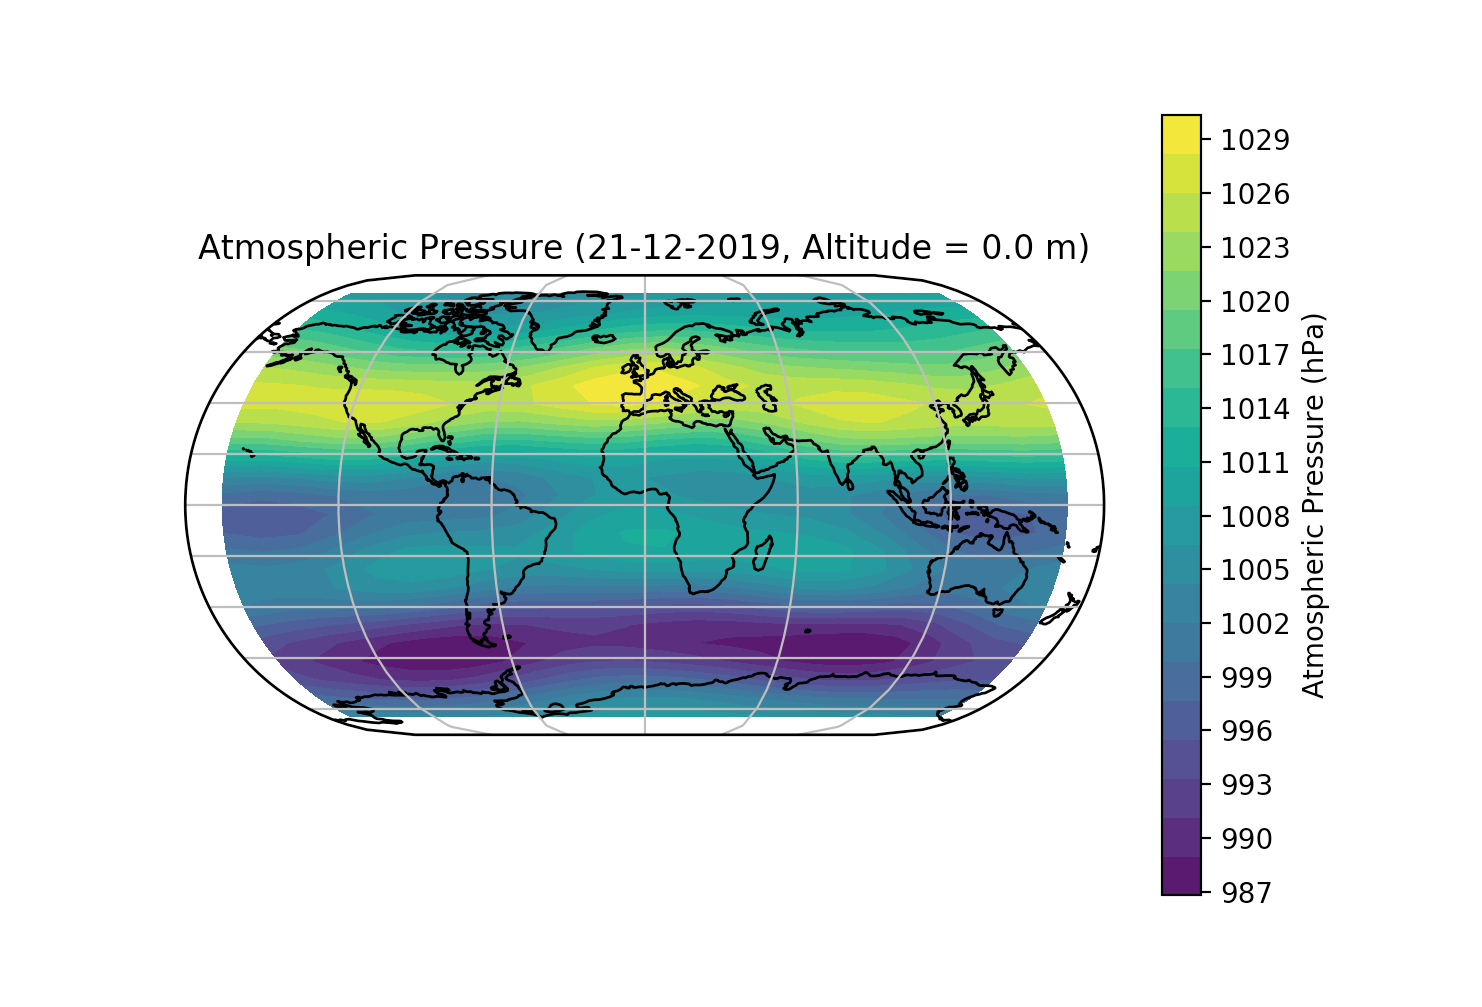
\includegraphics[width=.8\linewidth]{Graphs/contour_plots/pressure.png}
        \caption{Atmospheric Pressure Contour Plot}
    \end{figure}
    
    \begin{figure}[H]
        \centering
        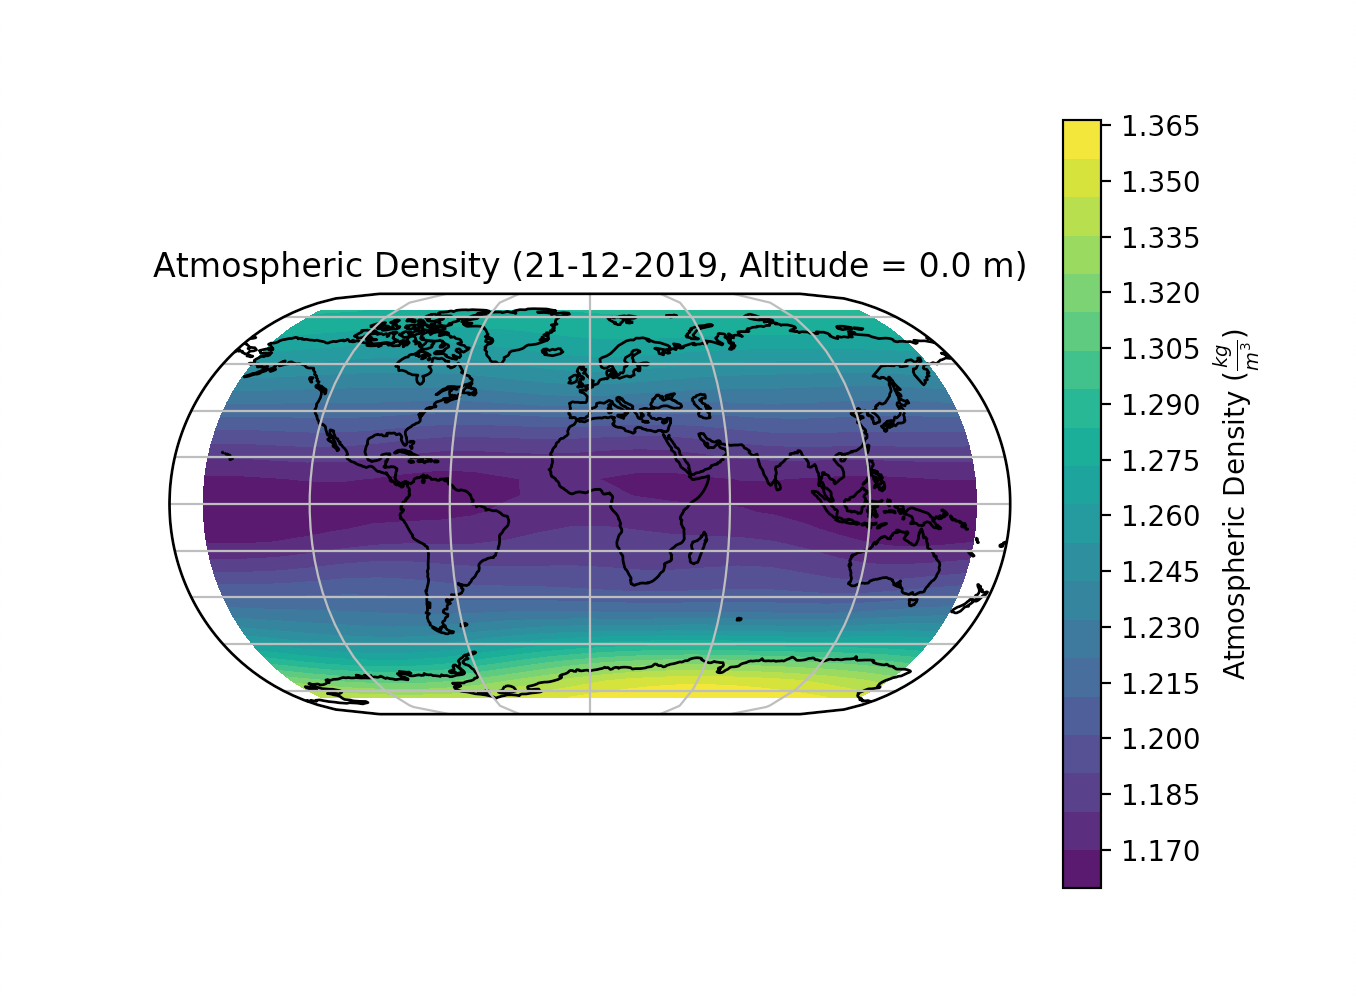
\includegraphics[width=.8\linewidth]{Graphs/contour_plots/density.png}
        \caption{Atmospheric Density Contour Plot}
    \end{figure}
    
    \begin{figure}[H]
        \centering
        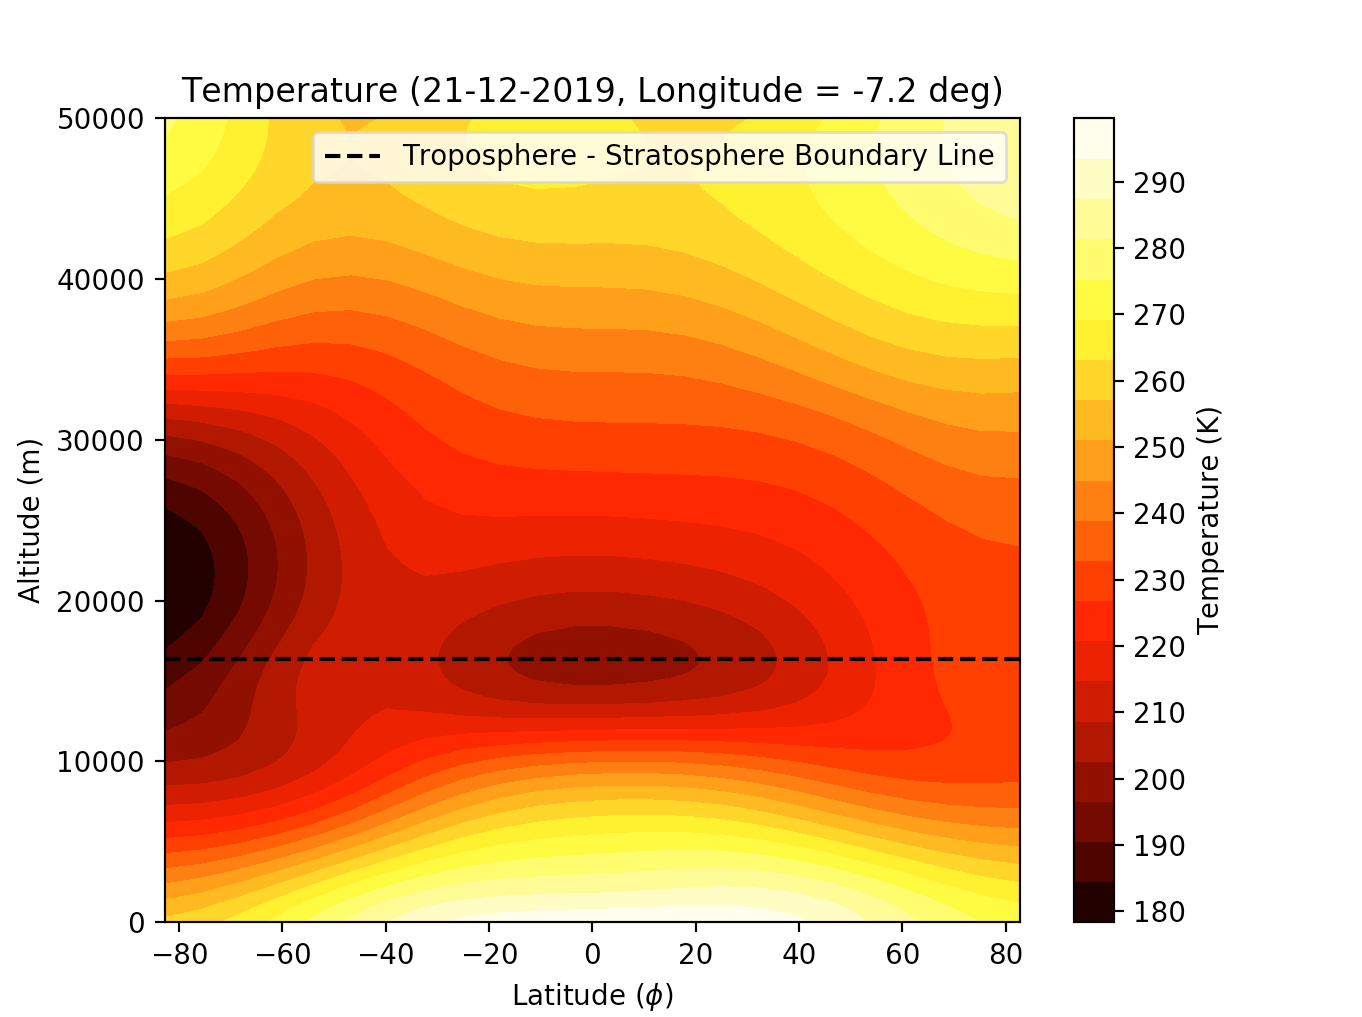
\includegraphics[width=.8\linewidth]{Graphs/contour_plots/temperature.png}
        \caption{Temperature Contour Plot}
    \end{figure}
    
    \subsection{Wind Class}
    \begin{figure}[H]
        \centering
        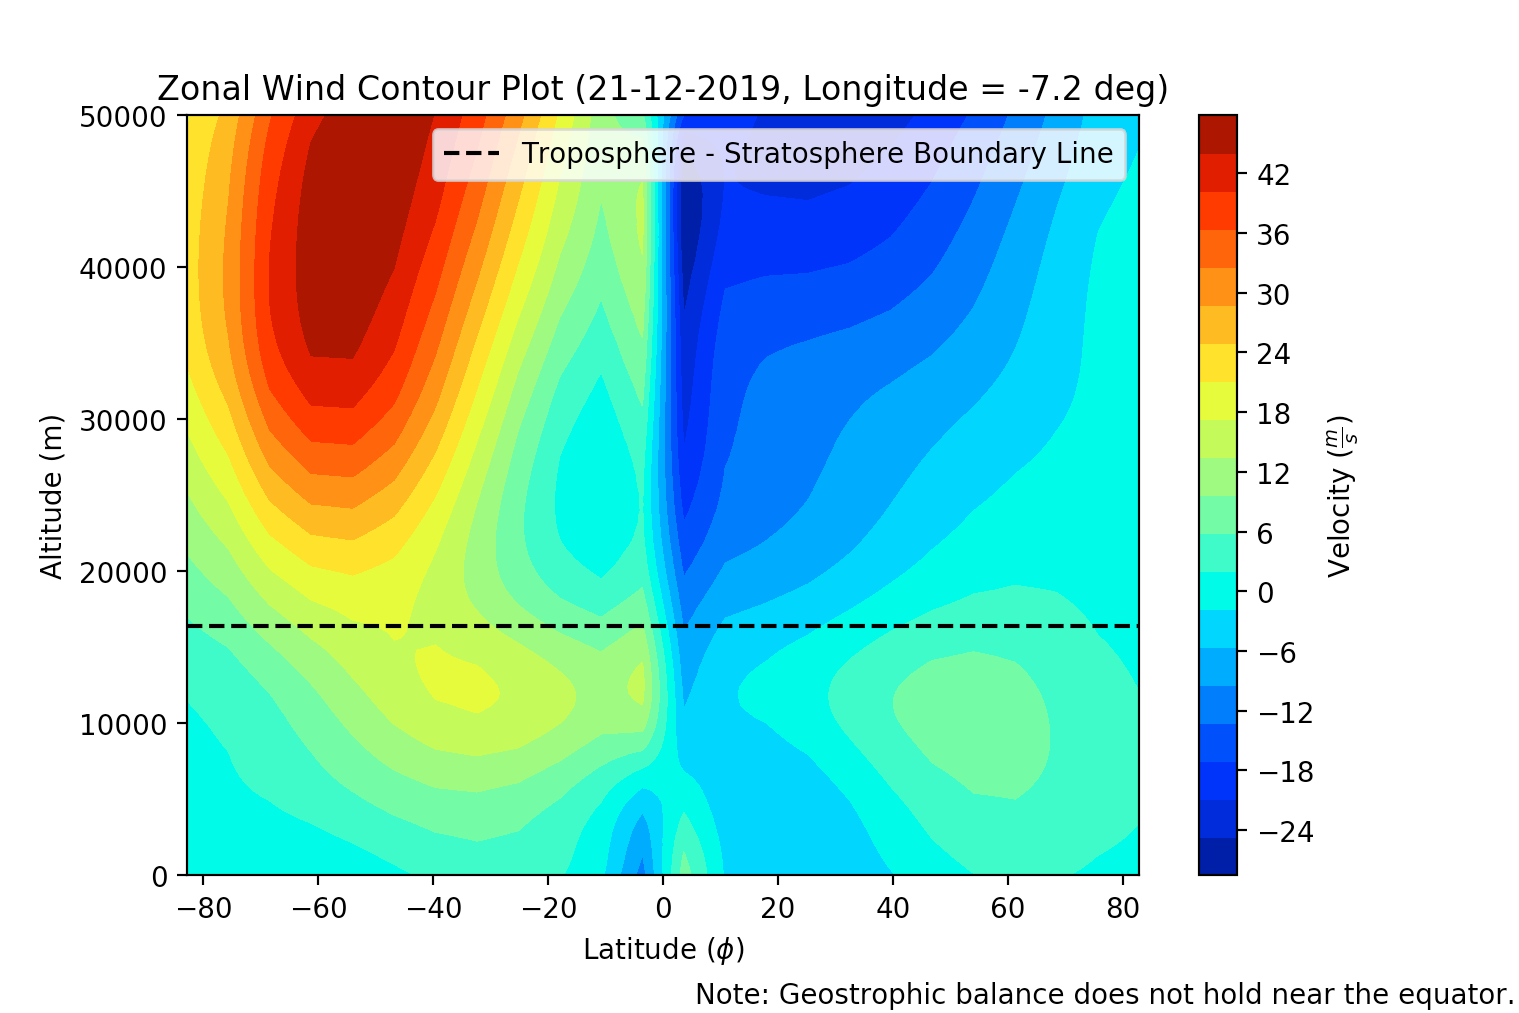
\includegraphics[width=.8\linewidth]{Graphs/contour_plots/zonal_wind.png}
        \caption{Zonal Wind Contour Plot}
    \end{figure}
    
    \begin{figure}[H]
        \centering
        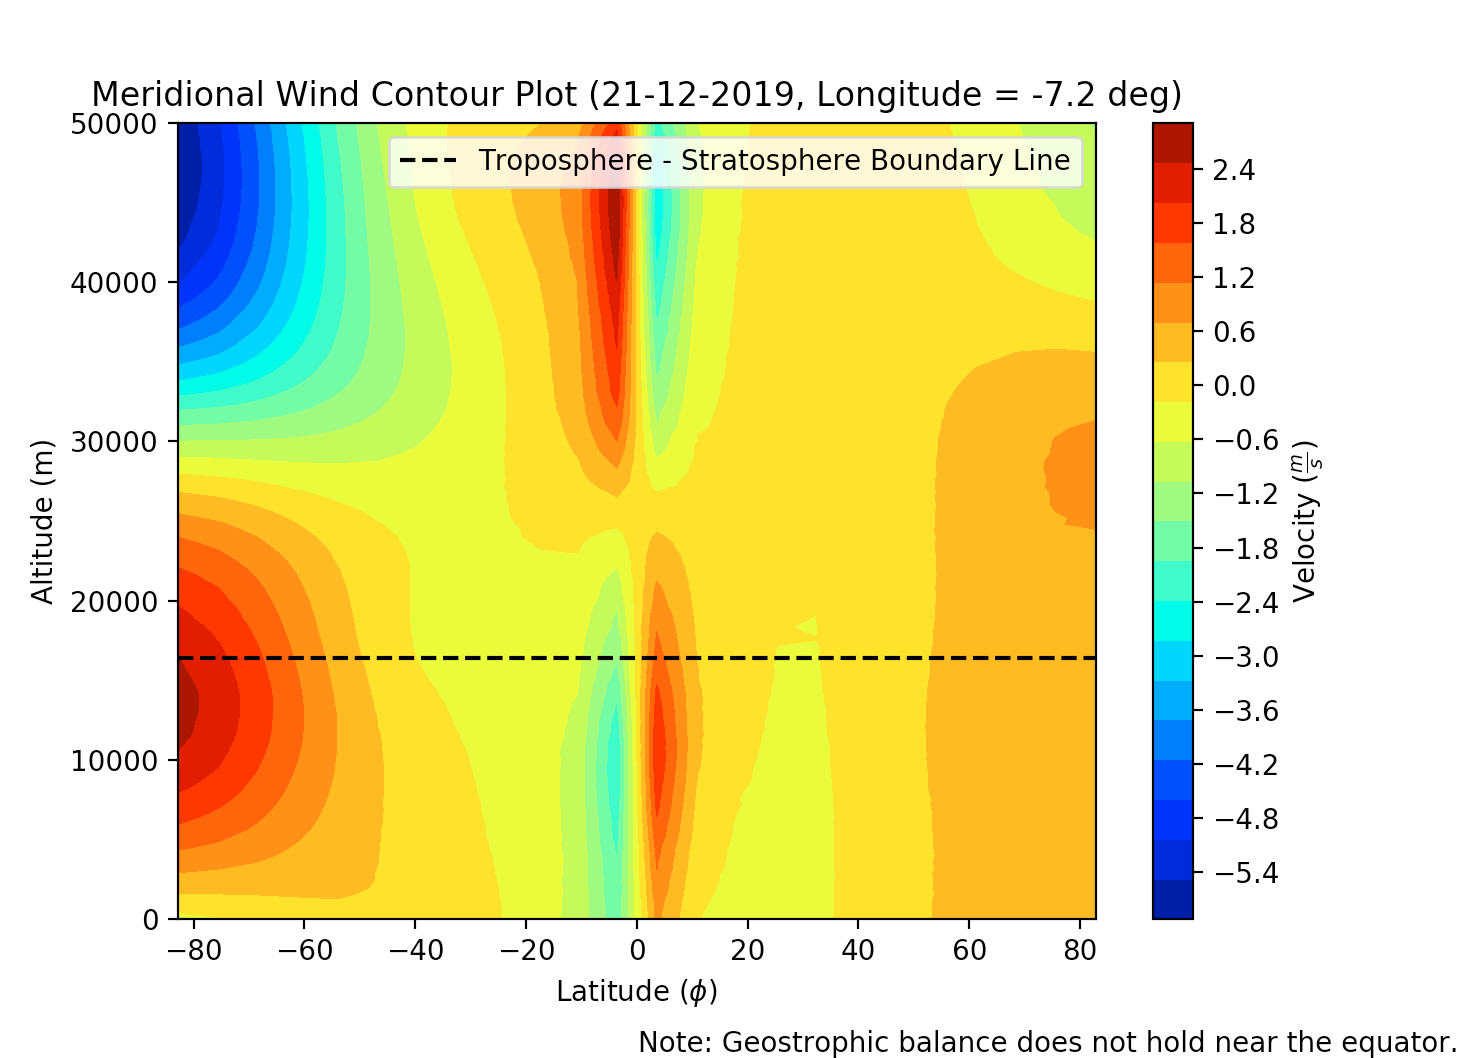
\includegraphics[width=.8\linewidth]{Graphs/contour_plots/meridional_wind.png}
        \caption{Meridional Wind Contour Plot}
    \end{figure}
    
    \begin{figure}[H]
        \centering
        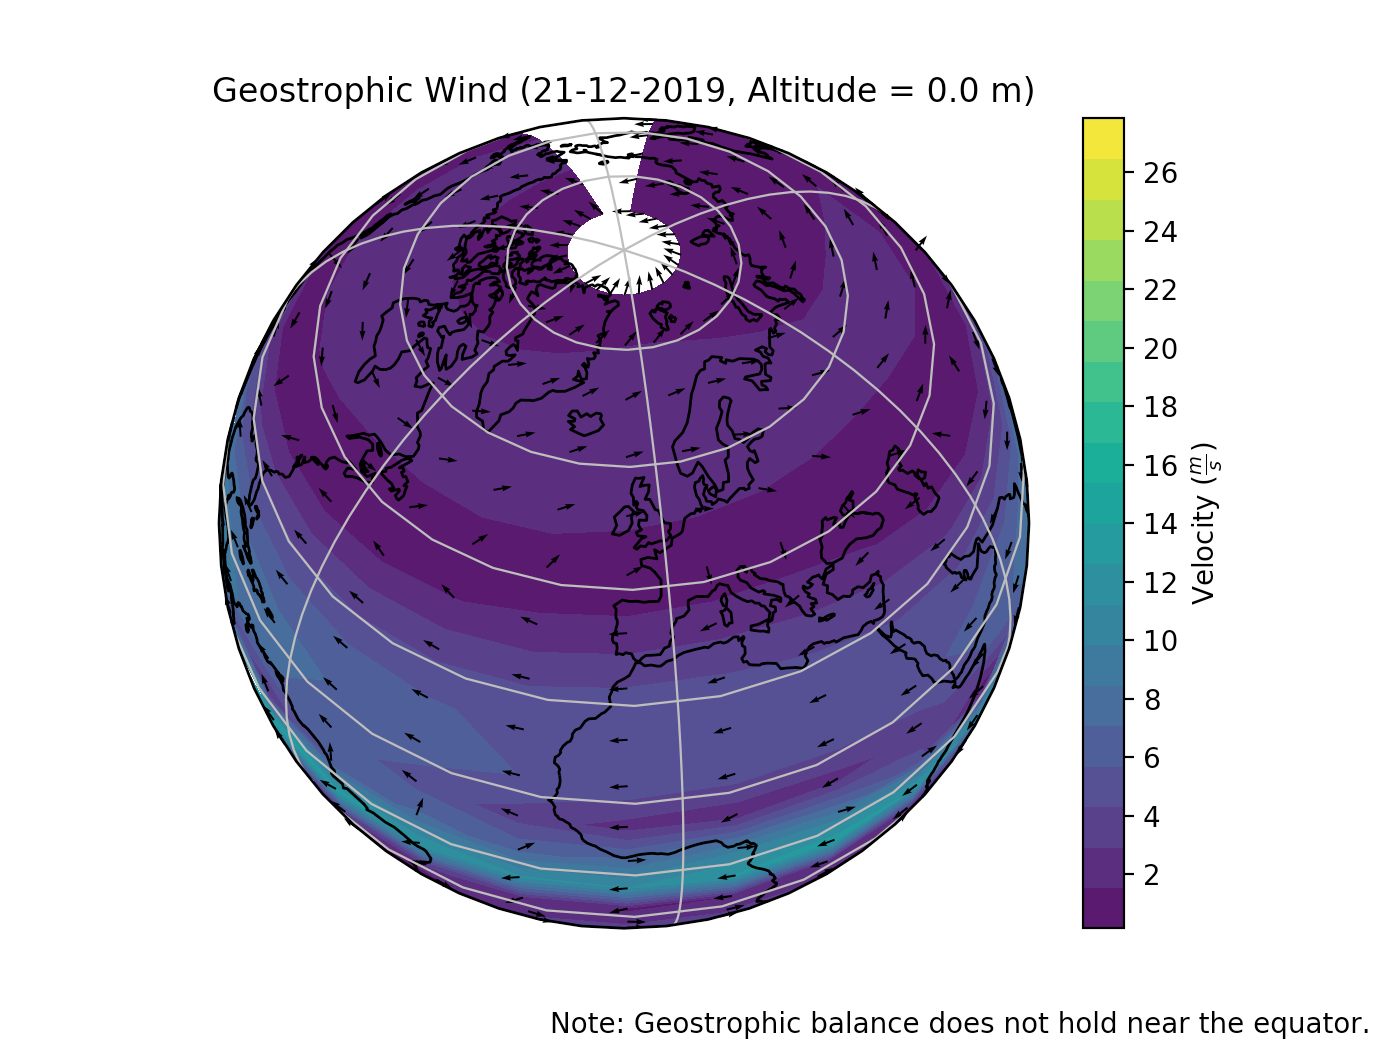
\includegraphics[width=.8\linewidth]{Graphs/contour_plots/globe.png}
        \caption{Geostrophic Wind (Globe View) Contour Plot}
    \end{figure}
    
    \subsection{Water and Dynamics Class}
    \begin{figure}[H]
        \centering
        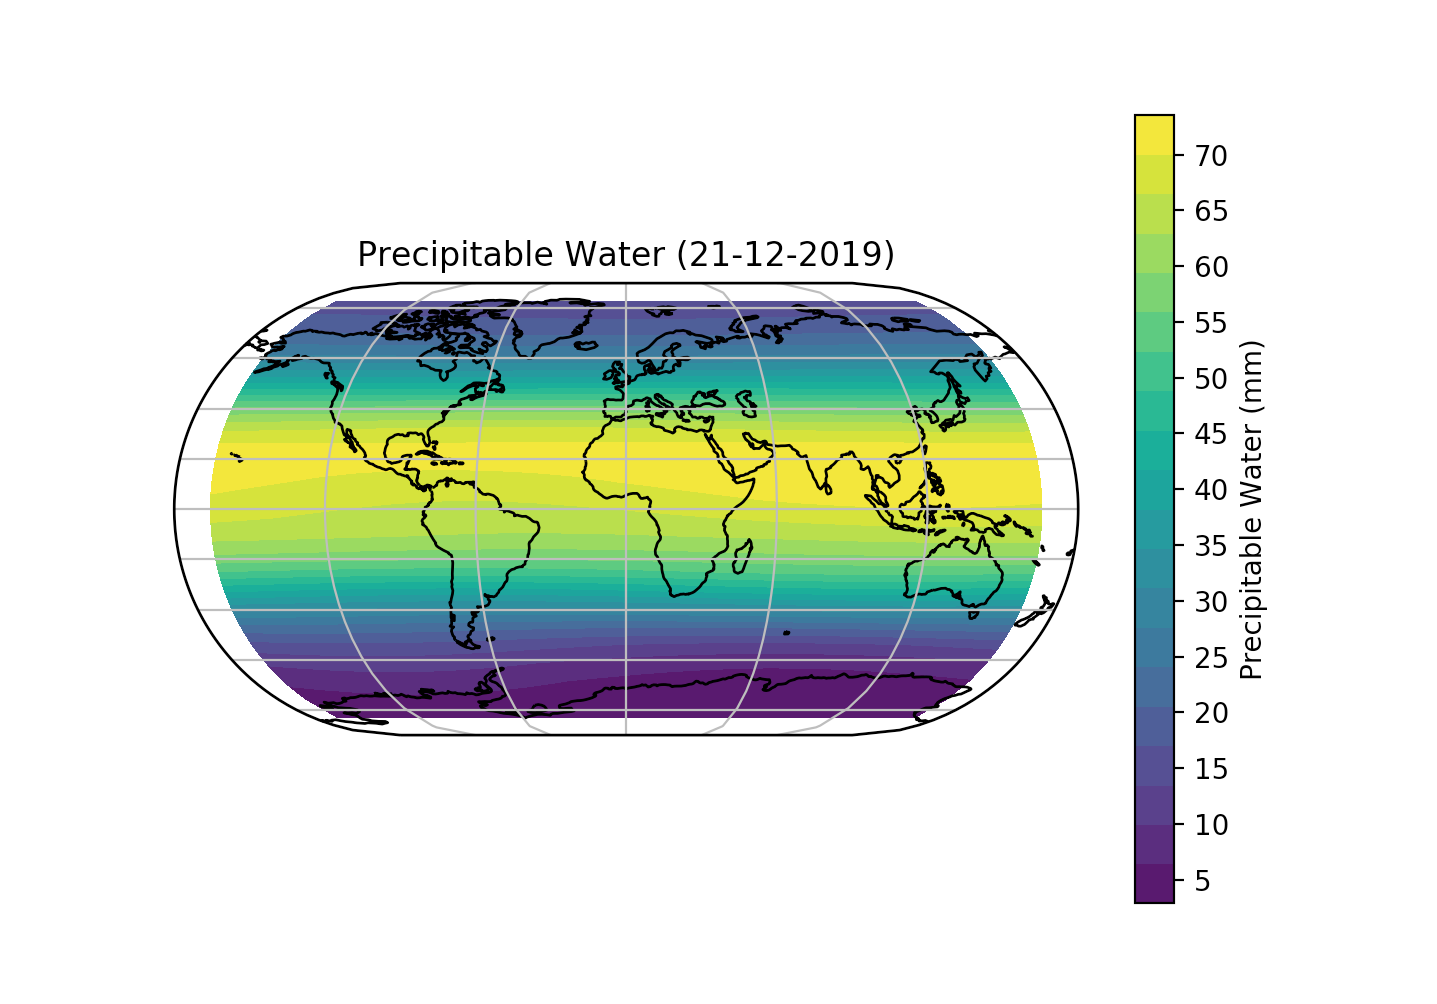
\includegraphics[width=.8\linewidth]{Graphs/contour_plots/precipitable_water.png}
        \caption{Precipitable Water Contour Plot}
    \end{figure}
    
    \begin{figure}[H]
        \centering
        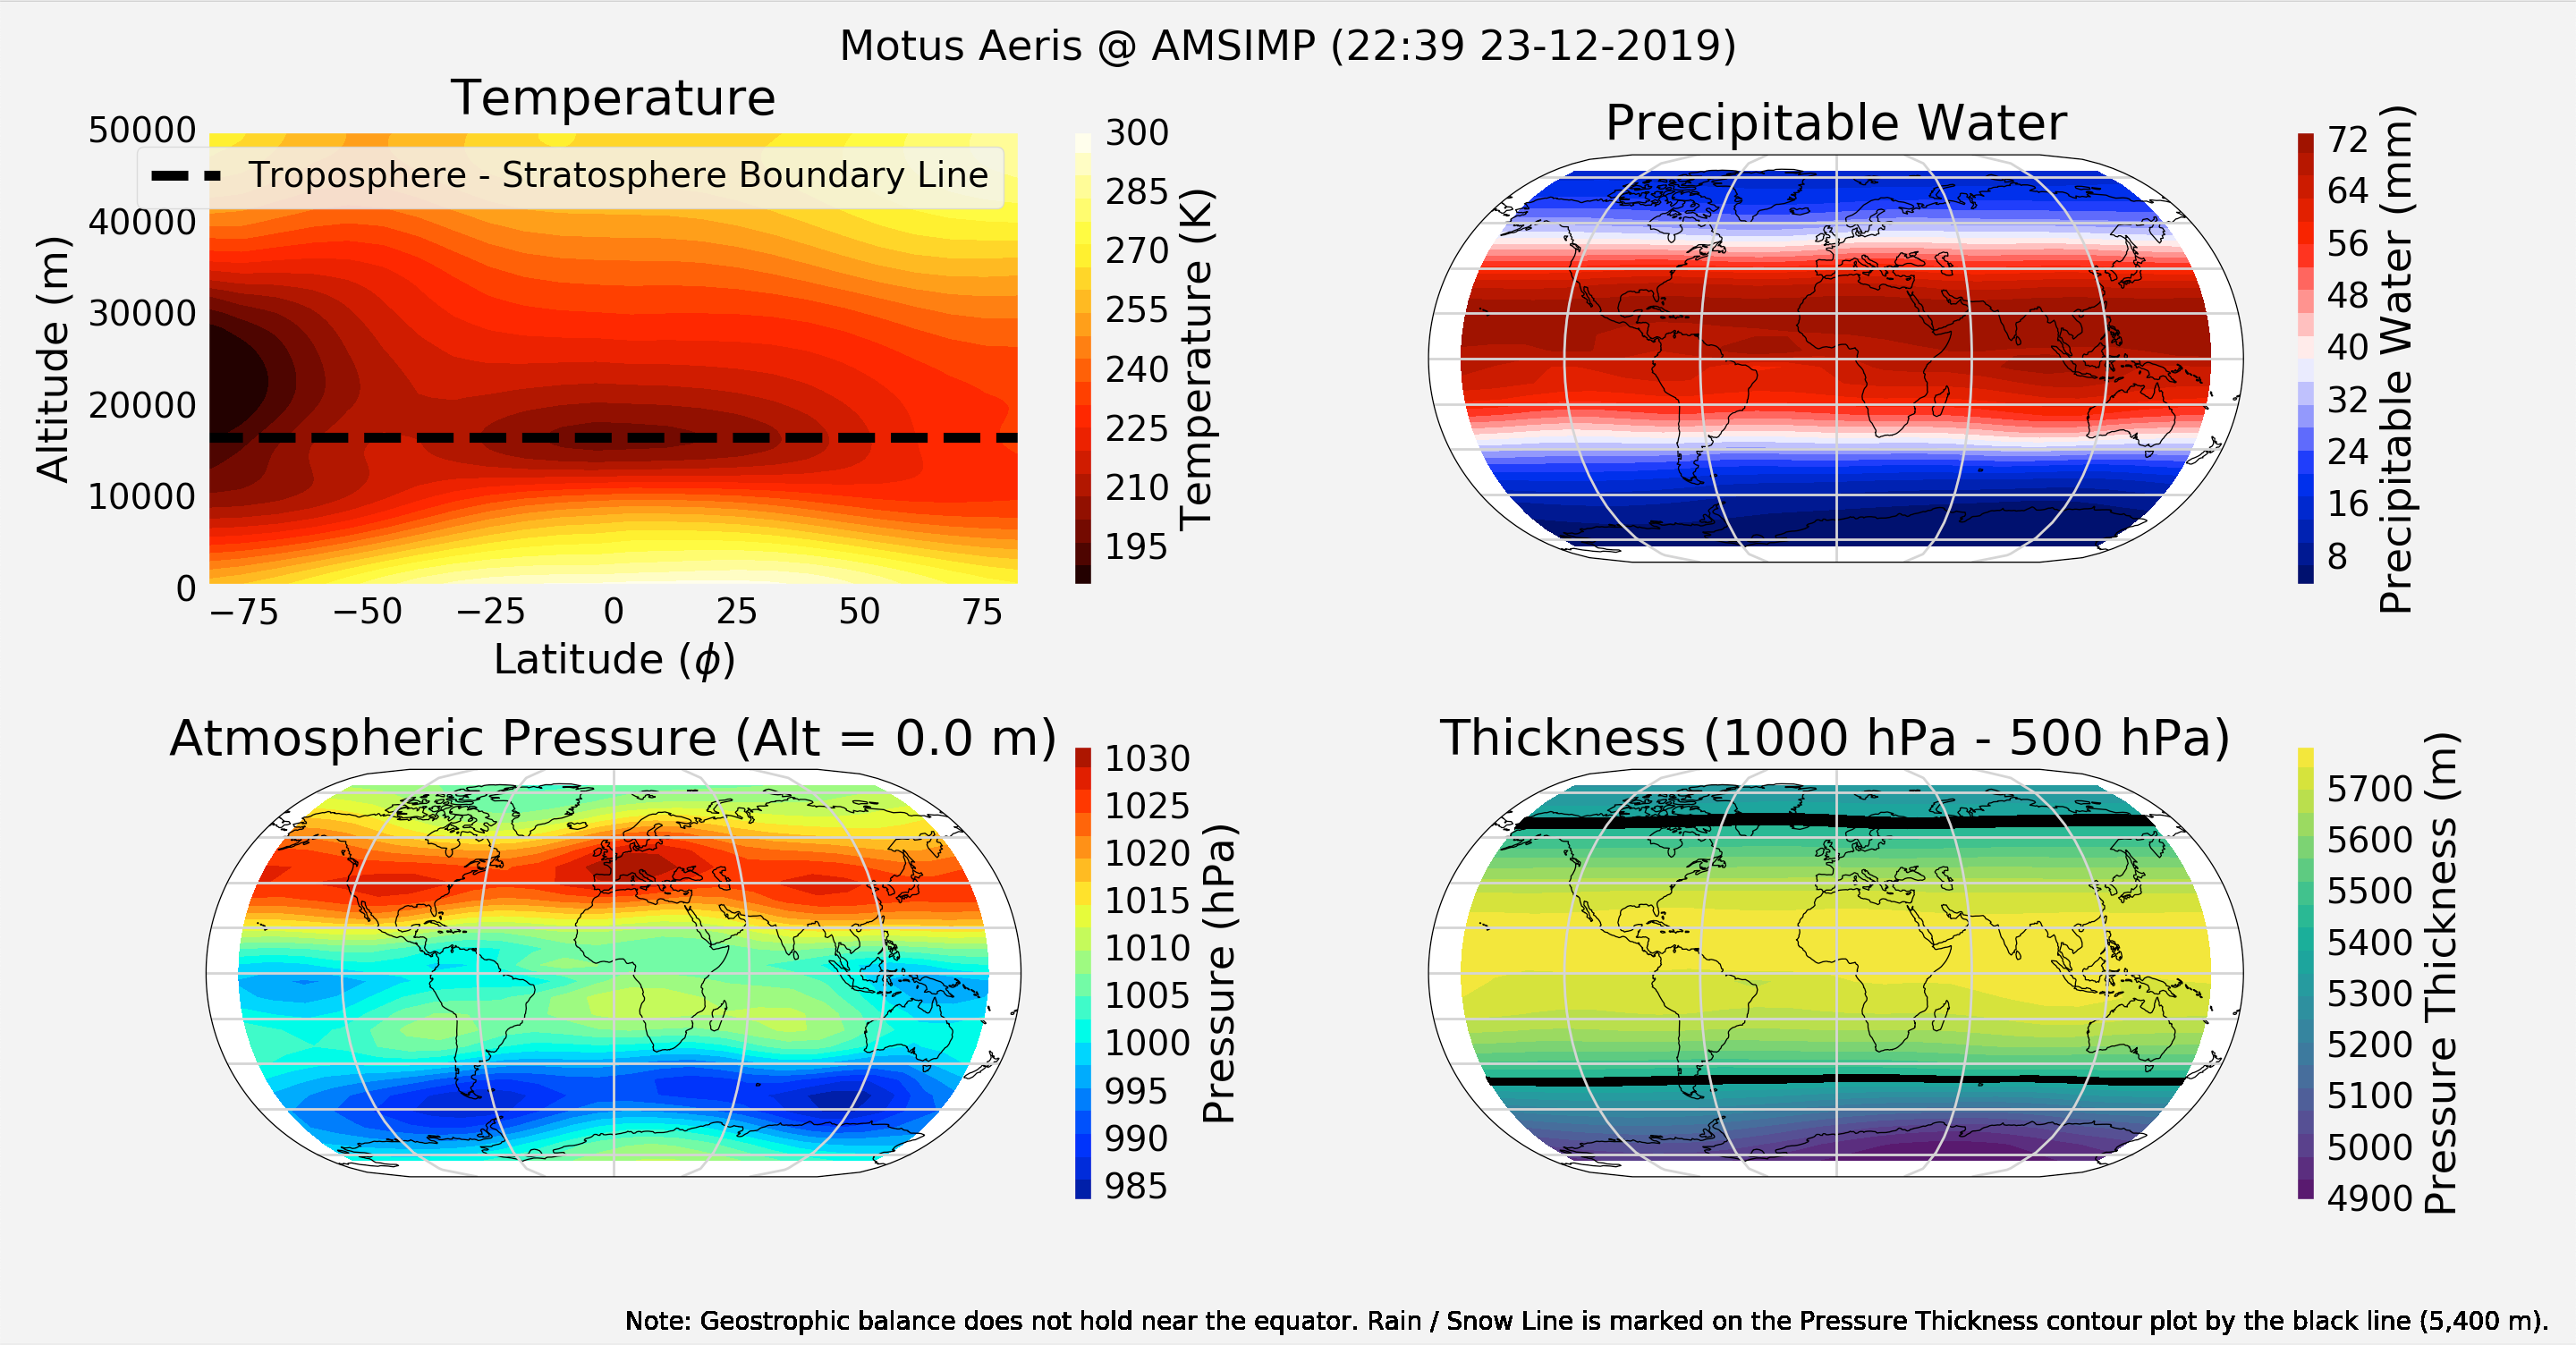
\includegraphics[width=.8\linewidth]{Graphs/contour_plots/forecast.png}
        \caption{Motus Aeris @ AMSIMP}
    \end{figure}
\end{appendices}